\section{Canonical Response Is Not Semantic Equivalence}
\label{sec:language}

\subsection{Canonical LEFT/RIGHT response}

All 324 canonical LEFT/RIGHT pairs across the eight completed rows execute different action sequences: 135 DROID/RoboLab pairs and 189 RoboTwin pairs. Endpoint ordering is positive in $125/135$ and $128/189$ pairs, respectively. These observations reject the narrow hypothesis that changing the canonical direction token leaves control unchanged. They do not show that the policy represents the relation independently of the wording, nor do they guarantee task completion.

A fixed-observation diagnostic issued 336 action requests without executing the robot; all 12 exact repeats were bit-identical. For $\pi_{0.5}$, prompt-induced action difference was about $4\%$ of cross-seed same-prompt variation but aligned across seeds. Cosmos3 Nano showed a larger, less consistently oriented effect, while DreamZero had no same-prompt variation. These open-loop rankings did not match closed-loop endpoint ordering, so action difference is a positive control, not a standalone grounding score.

\subsection{Reference inversion}

C002 asks whether the same physical relation is preserved when expressed from the other object's frame. Under inversion, the surface direction word and physical goal point in opposite directions. Relation preservation therefore predicts a positive physical-LEFT-minus-physical-RIGHT endpoint contrast. A simple template-invariant direction-token rule instead predicts a negative contrast---$-23.28$\,cm if the canonical response magnitude transferred unchanged.

Fig.~\ref{fig:c002} shows that neither idealized response occurs. Canonical prompts separate the endpoints by $+23.28$\,cm (95\% CI $[21.89,24.56]$), whereas reference-inverted prompts yield only $+0.19$\,cm ($[-0.88,1.27]$). The directional endpoint response therefore collapses under inversion: it provides neither reliable relation-consistent ordering nor evidence for simple canonical-scale token mirroring. This conclusion is specific to endpoint direction, not all prompt sensitivity; all 682 canonical/inverted physical-goal pairs execute different action traces.

\begin{figure}[t]
  \centering
  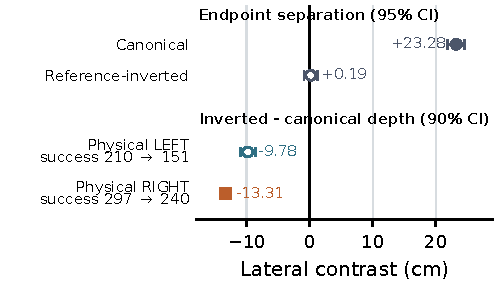
\includegraphics[width=0.98\columnwidth]{figures/reference_inversion.pdf}
  \caption{\textbf{Reference inversion collapses directional endpoint separation for $\pi_{0.5}$.}
  Top: physical-LEFT-minus-physical-RIGHT endpoint separation with seed-clustered 95\% bootstrap intervals; positive is relation-consistent. Bottom: inverted-minus-canonical requested-side depth with 90\% intervals; labels give canonical-to-inverted success counts out of 341. C002 seeds 12000--12340 are independent of E004.}
  \label{fig:c002}
\end{figure}

Within each physical goal, inversion also reduces placement depth. The inverse-minus-canonical change is $-9.78$\,cm for physical LEFT (90\% CI $[-10.92,-8.59]$) and $-13.31$\,cm for physical RIGHT ($[-14.07,-12.54]$); both intervals lie outside the registered $\pm4.15$\,cm equivalence margin. Success falls from $210/341$ to $151/341$ for LEFT and from $297/341$ to $240/341$ for RIGHT. The corresponding changes, $-17.30$ and $-16.72$ percentage points, do not meet the registered $\pm15.56$-point equivalence criterion. The inverse endpoint-ordering control also fails, so the semantic-equivalence claim is withheld. Canonical response is therefore insufficient evidence that a physical relation is preserved across reference frames.
